\chapter{Virtuelle LANs}

Virtuelle Netze oder auch virtuelle local area networks (VLAN) werden genutzt, um bestehende physische LANs in logische Abschnitte zu Unterteilen, oder auch um mehrere physische Netzabschnitte virtuell zu verbinden. VLANs werden mithilfe von Switches gebildet. Switche sind Netzwerkkomponenten, welche die Schichten eins und zwei des Internetprotokollstapels (vgl. Anhang \ref{A1}) implementieren, sie bilden heute die Zentralen Netzknoten in (lokalen) Netzwerken \cite{zisler2018computer}. 

%nutzen hinzufügen

\subsection{Funktionsweise}

% portbasiertes und tagged Vlan

Es gibt zwei Arten von Vlans, das portbasierte und das paketbasierte VLAN. 
Bei dem in Abbildung \ref{vlanport} dargestellten portbasiertem VLAN, wir jeder Port eines Switches einem VLAN zugewiesen. Soll nun eine Kommunikation zwischen den Geräten, die a VLAN A angeschlossen sind und jenen aus VLAN B stattfinden, müssen jeweils ein Port aus VLAN A mit einem aus VLAN B per Kabel verbunden werden \cite{zisler2018computer}. % Verbindung muss über einen Router laufen?? 


\begin{figure}[h]
\centering
	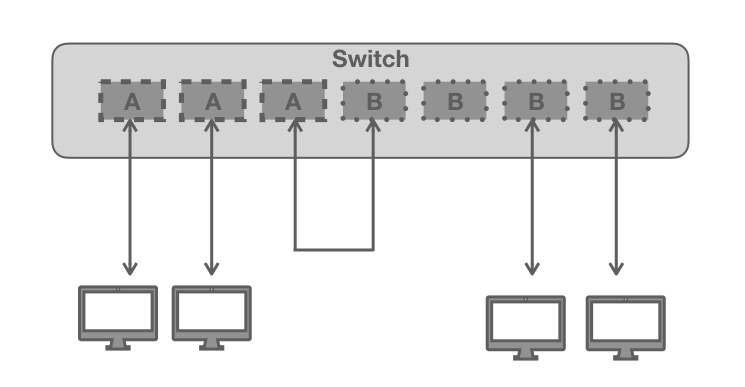
\includegraphics[width=0.8\linewidth, height= 6cm]{vlanport.001.png}
	\caption{Portbasiertes VLAN}
	\label{vlanport}
\end{figure}


Das in Abbildung \ref{vlanpak} gezeigte Paketbasierte VLAN, auch \emph{tagged VLAN}, ermöglicht es, dass ein Port auch mehreren VLANs zugeordnet werden kann. Bei  diese Art des virtuellen Netzes können zwei (oder mehr) VLANs, die über zwei (oder mehr)  Switche verteilt sind mit nur einem Kabel verbunden werden, wofür sonst zwei Kabel und je Switch zwei Ports verwendet werden müssten. Die Verbindung zwischen zwei Switches über die mehrere VLANs laufen wird Trunk genannt \cite{cisco14rout}. 

  Die Zugehörigkeit der Pakete zu einem VLAN wird über einen VLAN-Tag nach dem Standard  IEEE 802.1Q am Ehternet-Frame gekennzeichnet. 

\begin{figure}[h]
\centering
	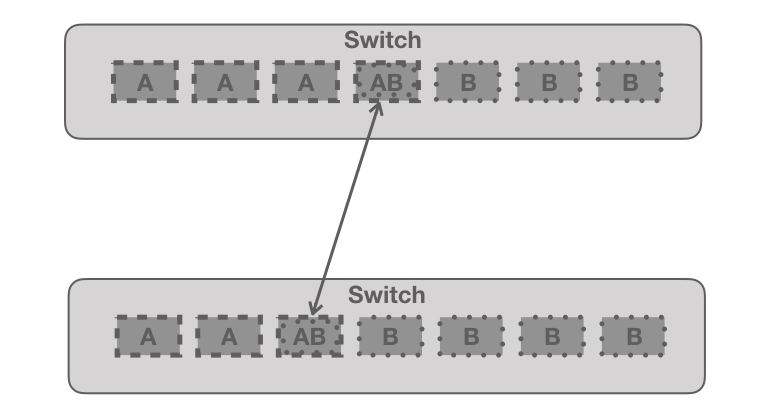
\includegraphics[width=0.8\linewidth,height=6cm]{vlanpak.001.jpeg}
	\caption{Paketbasiertes VLAN}
	\label{vlanpak}
\end{figure}


